\documentclass[12pt,fleqn]{article}
\usepackage[utf8]{inputenc}
\usepackage[inline]{enumitem}
\usepackage[margin=2cm]{geometry}
\usepackage{amsmath}
\usepackage{tikz}
\usepackage{amsfonts}

\date{}
\title{\textbf{Pitkän matematiikan kertaus}}
\author{Jimi Käyrä}

\begin{document}
\begin{titlepage}
\maketitle
\thispagestyle{empty}
\end{titlepage}

\section*{1. kurssi: Luvut ja lukujonot}
\begin{enumerate}[label=\textbf{\arabic*.}]
\item 
\begin{enumerate}[label=\textbf{\alph*)}]
\item Laske \(\displaystyle 1\frac{2}{3}:2\frac{1}{2}\).
\item Sievennä lauseke \(\displaystyle \frac{2^{100}}{4^{50}}\).
\item Määritä luvun \(a\) vastaluvun ja luvun \(b^{-1}\) käänteisluvun tulo.
\item Osoita, että luvut \(\sqrt{2}\) ja \(\displaystyle \frac{\sqrt{2}}{2}\) ovat toistensa käänteislukuja.
\end{enumerate}


\item Määritä luku \(a\) siten, että yhtälö \(ax - 3x + 3a + 1 = 0\) ei toteudu millään \(x\):n reaalilukuarvolla.

\item Ratkaise yhtälöt ja epäyhtälö.
\begin{enumerate}[label=\textbf{\alph*)}]
\item \(\displaystyle \frac{3x}{4}+\frac{x}{3}=1\)
\item \(2^{4x}=16\)
\item \(\displaystyle 4\cdot 2^x=\frac{1}{32}\)
\item \(2\left(x-1\right)-3\left(x+1\right)\leq 1\)
\end{enumerate}

\item Tuoreissa omenissa on 4 \% sokeria ja 80 \% vettä. Omenat kuivatetaan siten, että niiden uusi vesipitoisuus on 10 \%. Mikä on kuivien omenoiden sokeriprosentti?

\item Vuokra muodostaa 5 \% opiskelijan kuukausimenoista. Vuokraa korotetaan 2 \%.
\begin{enumerate}[label=\textbf{\alph*)}]
\item Kuinka monta prosenttiyksikköä vuokran osuus kuukausimenoista kasvaa?
\item Kuinka monta prosenttia opiskelijan on pienennettävä muita menojaan, jotta kokonaismenot pysyvät samoina?
\end{enumerate}

\item 
\begin{enumerate}[label=\textbf{\alph*)}]
\item Määrittele \emph{aritmeettinen jono} matemaattisesti.
\item Määritä vakio \(x\) siten, että jono \(x, 2x-1, 3x, ...\) on aritmeettinen.
\end{enumerate}

\item Aritmeettiselle jonolle \((a_n)\) pätee \(a_2=4\) ja \(a_5=10\). Määritä \(S_{100}\).

\item Bakteeriviljelmässä oli 2 000 bakteeria kello 13.00. Bakteerien määrä kasvaa 3,5 \% minuutin välein. Mihin kellonaikaan mennessä bakteerien määrä ylittää miljoonan rajan?

\item Keksi rekursiivinen sääntö jonon \(1, 2, 4, 7, 11, ...\) yleiselle jäsenelle.

\item Määritä \(\displaystyle \sum_{n=1}^{100} {\frac{1}{2^n}}.\)
\newpage
\section*{2. kurssi: Polynomifunktiot- ja yhtälöt}

\item Määritellään polynomit \(P(x)=x-1\) ja \(Q(x)=x^2+1\).
\begin{enumerate}[label=\textbf{\alph*)}]
\item Määritä \(P(x)-Q(x)\).
\item Laske \(P(x)\cdot Q(x)\).
\item Sievennä lauseke \(P(x)^2\).
\end{enumerate}

\item 
\begin{enumerate}[label=\textbf{\alph*)}]
\item Miten neliöjuuri määritellään?
\item Tutki, onko \(\sqrt{4-4\sqrt{5}}=2(1-\sqrt{5})\).
\item Sievennä lauseke \(\sqrt{(1-2\pi)^2}+\sqrt{8}\).
\end{enumerate}

\item Jaa polynomi mahdollisimman matalaa astetta oleviin tekijöihin.
\begin{enumerate}[label=\textbf{\alph*)}]
\item \(4x^2-16\)
\item \(x^3-x^2+3x-3\)
\item \(4x^2-4x+1\)
\end{enumerate}

\item Supista murtolauseke \(\displaystyle \frac{x^2-3x-4}{x-4}\).

\item Ratkaise yhtälö ja epäyhtälöt.
\begin{enumerate}[label=\textbf{\alph*)}]
\item \(x^3+0,008=0\)
\item \(2x^2-x\geq 3\)
\item \(x^3-x < 0\)
\end{enumerate}

\item Toisen asteen polynomi \(f(x)=2ax^2+x-1\) on jaollinen binomilla \(x-1\). Määritä polynomin nollakohdat.

\item Tarkastellaan funktiota \(f(x)=tx^3+2x^2+x\).
\begin{enumerate}[label=\textbf{\alph*)}]
\item Määritä funktion nollakohdat, kun \(t=1\).
\item Määritä \(t\) siten, että funktiolla on kolme eri suurta nollakohtaa.
\end{enumerate}

\item Määritä vakio \(a\) siten, että funktioiden \(f(x)=ax^2+4x-1\) ja \(g(x)=x^2+x-a\) kuvaajat sivuavat toisiaan, ts. niillä on yksi yhteinen piste.

\item Koirille rakennetaan suorakulmion muotoinen aitaus siten, että yhtenä sivuna on talon seinä. Aitamateriaalia on käytettävissä enintään 60 m ja aitauksen pinta-alan on oltava 100 m\(^2\). Määritä aitauksen kaikki mahdolliset mitat.

\item Erään tilaston mukaan vuonna 1995 Internetin käyttäjiä oli 0,4 \% maailman väestöstä. Vuonna 2017 vastaava tunnusluku oli 49,6 \%. Kuinka suuri oli Internetin käyttäjämäärän keskimääräinen vuosittainen kasvuprosentti tällä aikavälillä? Maailman väestö kasvoi noin 30 \% kyseisellä aikavälillä.

\item Reaaliluku on \emph{algebrallinen}, jos se on jonkin kokonaislukukertoimisen polynomin nollakohta. Tällaiset polynomit ovat muotoa
\[P(x)=a_0+a_1 x+a_2 x^2+...+a_n x^n,\]
kun polynomin asteluku on \(n=1,2,3,...\) ja kertoimet \(a_0,a_1,a_2,...,a_n\) ovat kokonaislukuja. Osoita, että luku \(x\) on algebrallinen johtamalla jonkin sopivan polynomin lauseke, kun
\begin{enumerate}[label=\textbf{\alph*)}]
\item \(\displaystyle x=\frac{2}{3}\)
\item \(\displaystyle x=\sqrt{3}\)
\item \(\displaystyle x=2+\sqrt{3}\)
\item \(\displaystyle x=\sqrt{2}+\sqrt{3}\). \emph{(yo s16)}
\end{enumerate}
\newpage
\section*{3. kurssi: Geometria}

\item 
\begin{enumerate}[label=\textbf{\alph*)}]
\item Kolmion sivujen pituudet ovat 2, \(\sqrt{10}\) ja \(2\sqrt{2}\). Onko kolmio suorakulmainen?
\item Kolmion pinta-ala on 2 cm\(^2\), ja sen vierekkäisten sivujen pituudet ovat 2 cm ja 3 cm. Kuinka suuri on näiden sivujen välinen kulma?
\end{enumerate}

\item Lukua \(\pi\) voidaan approksimoida asettamalla ympyrän sisään säännöllinen monikulmio, jonka kärjet ovat ympyrän kehällä. Tällöin likiarvo saadaan monikulmion piirin ja ympyrän säteen suhteena. Kuinka monen desimaalin tarkkuudella saadaan luvun \(\pi\) arvo, kun sitä approksimoidaan säännöllisellä 96-kulmiolla?

\item Kolme euron kolikkoa asetetaan sivuamaan toisiaan. Laske kolikkojen väliin jäävän alueen pinta-ala, kun euron kolikon halkaisija on 23,25 mm.

\item Osoita, että säännöllisen \(n\)-kulmion kulmien summa on \((n-2)\cdot 180^{\circ}\).


\item Täysin pyöreän geenimanipuloidun omenan säde on 5,0 cm. Omenan läpi porataan sen keskeltä kulkeva reikä, jonka säde on 1,0 cm. Kuinka monta prosenttia omenan tilavuudesta tällöin häviää? Anna vastaus prosenttiyksikön kymmenesosan tarkkuudella. \emph{(yo s15)}

\item Laske kolmion \(ABC\) pinta-alan tarkka arvo.

\begin{tikzpicture}
\draw[black,thick] (0,0) -- (10,0) -- (7,4.5) -- cycle;
\draw[black,thick,dashed] (7,0) -- (7,4.5);
\end{tikzpicture}

\item Ympyräkartion pohjan säde on 1 ja korkeus 2. Sen sisään asetetaan pallo, joka sivuaa kartion pohjaa ja vaippaa. Määritä pallon säde.

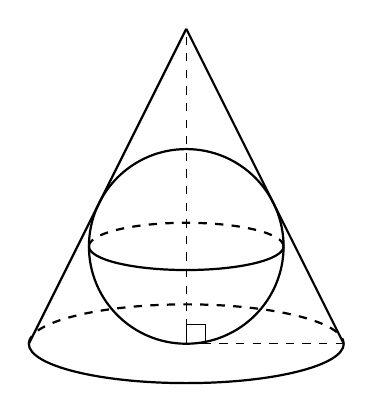
\begin{tikzpicture}

\draw[black,dashed] (0,0) -- (0,4);
\draw[black,dashed] (0,0) -- (2,0);
\draw[black] (0,0) rectangle (0.25,0.25);

\draw[black,thick,dashed] (-2,0) arc (180:0:2cm and 0.5cm);
 \draw[black,thick] (-2,0) arc (180:360:2cm and 0.5cm);
\draw[black,thick] (-2,0) -- (0,4);
\draw[black,thick] (2,0) -- (0,4);

\draw[black,thick] (0,1.23606798) circle (1.23606798 cm);

\draw[black,thick,dashed] (-1.23606798,1.23606798) arc (180:0:1.23606798cm and 0.3cm);
 \draw[black,thick] (-1.23606798,1.23606798) arc (180:360:1.23606798cm and 0.3cm);
 


\end{tikzpicture}

\item Paikat \(A\) ja \(B\) sijaitsevat molemmat leveyspiirillä \(50^{\circ}\), ja niiden pituusasteiden erotus on \(20^{\circ}\). Mikä on paikkojen välinen etäisyys? Entä kuinka pitkä olisi paikasta \(A\) paikkaan \(B\) porattu suora tunneli?

\item \(\mathrm{CH}_4\)-molekyylin neljä vetyatomia ovat säännöllisen tetraedrin kärjissä, ja hiiliatomi on tetraedrin korkeusjanalla yhtä etäällä kaikista vetyatomeista. Määritä metaanimolekyylin sidoskulma, ts. kahdesta vetyatomista hiiliatomiin vedettyjen janojen välinen kulma.\\
\emph{(Vihje: Korkeusjana leikkaa tetraedrin pohjan sen painopisteessä.)}
\item Kuinka kauas on mahdollista nähdä 1 km korkeasta tornista? Maapallon säde on 6 370 km.

\item Vesisäiliön, jonka mitat on ilmoitettu kuviossa, veden korkeudeksi mitattiin 10 cm. Kuinka paljon säiliössä on vettä?
\newpage
\section*{4. kurssi: Vektorit}

\item Kuviossa on esitetty vektorit \(\bar{a}, \bar{b}\) ja \(\bar{c}\).

\begin{enumerate}[label=\textbf{\alph*)}]
\item Piirrä vektorit \(\bar{a}-\bar{b}\) ja \(2\bar{a}+\bar{b}\).
\item Jaa vektori \(\bar{c}\) vektorien \(\bar{a}\) ja \(\bar{b}\) suuntaisiin komponentteihin piirtämällä.
\end{enumerate}

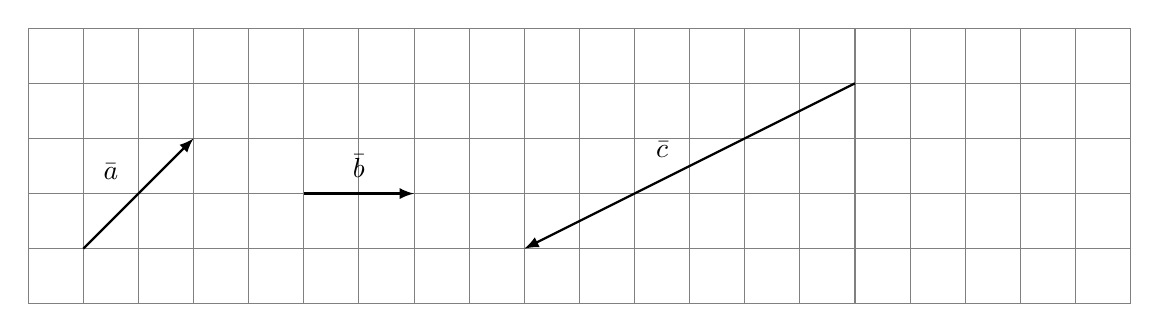
\begin{tikzpicture}[scale=0.7]
\draw[help lines, gray, thin] (0,0) grid (20,5);

\draw [-latex, black, thick] (1,1) -- (3,3);
\node at (1.5,2.4) {\(\bar{a}\)};

\draw [-latex, black, thick] (5,2) -- (7,2);
\node at (6,2.5) {\(\bar{b}\)};

\draw [-latex, black, thick] (15,4) -- (9,1);
\node at (11.5,2.8) {\(\bar{c}\)};

\end{tikzpicture}
\item Selitä käsite ja anna esimerkki.
\begin{enumerate}[label=\textbf{\alph*)}]
\item paikkavektori
\item tason vektoriyhtälö
\item komponenttiesityksen yksikäsitteisyys
\item vektorin \(\bar{a}\) suuntainen yksikkövektori
\end{enumerate}

\item Olkoot vektorit \(\bar{a}=10\bar{i}+3\bar{j}\) ja \(\bar{b}=3\bar{i}+t\bar{j}\), \(t \in \mathbb{R}\). Määritä \(t\) siten, että
\begin{enumerate}[label=\textbf{\alph*)}]
\item vektorit ovat yhtä pitkät,
\item vektorit ovat kohtisuorassa toisiaan vastaan,
\item vektorit ovat yhdensuuntaiset. Ovatko ne tällöin samansuuntaiset vai vastakkaissuuntaiset?
\end{enumerate}

\item Origosta \(O\) alkava vektori \(\overline{OP}\) on vektorin \(3\bar{i}+\bar{j}\) suuntainen, ja sen kärki \(P\) on pisteiden \(A=(1,2)\) ja \(B=(7,1)\) yhdysjanalla. Missä suhteessa piste \(P\) jakaa janan \(AB\)?\emph{ (yo s04)}

\item Vektorit \(\bar{a}\) ja \(\bar{b}\) ovat vastakkaissuuntaiset. Olkoon \(\bar{a}=\frac{3}{2}\bar{i}-2\bar{j}\) ja olkoon vektorin \(\bar{b}\) pituus 5. Määritä \(\bar{b}\). Mikä on loppupiste, kun \(\bar{b}\) asetetaan alkamaan pisteestä \((4,3)\)? \emph{(yo k01)}

\item Kolmiolla \(ABC\) on sivuvektorit \(\overline{AB}=\bar{i}+2\bar{j}+3\bar{k}\) ja \(\overline{AC}=2\bar{i}+\bar{j}-3\bar{k}\). 
\begin{enumerate}[label=\textbf{\alph*)}]
\item Piirä kolmio \(xyz\)-koordinaatistoon.
\item Määritä kolmion suurin kulma ja pinta-ala.
\end{enumerate}

\item Olkoon \(|\bar{a}|=1\) ja \(|\bar{b}|=\sqrt{2}\) ja \(\bar{a}\cdot \bar{b}=\frac{1}{2}\). Laske vektorien \(\bar{a}+\bar{b}\) ja \(\bar{a}-\bar{b}\) välinen kulma.

\item Suoraviivaisesti lentävä lentokone kulkee pisteiden \(A=(60,50,40)\) ja \(B=(10,5,20)\) kautta.
\begin{enumerate}[label=\textbf{\alph*)}]
\item Muodosta lentorataa kuvaavan suoran vektoriyhtälö.
\item Missä pisteessä kone koskettaa \(xy\)-tasoa?
\item Kuinka suuressa kulmassa kone kohtaa \(xy\)-tason?
\end{enumerate}

\item Taso kulkee origon ja pisteiden \((5,4,3)\) sekä \((10,2,5)\) kautta. Määritä tason yhtälö normaalimuodossa.

\item Taso sisältää suoran \(
\begin{cases}
x=2t \\
y=t+1 \\
z=3t-1
\end{cases},\) \(t\in \mathbb{R}\) ja pisteen \((1,2,3)\).
\begin{enumerate}[label=\textbf{\alph*)}]
\item Määritä tason yhtälö parametrimuodossa.
\item Mikä on origon etäisyys tasosta?
\end{enumerate}

\item Osoita, että puoliympyrän sisältämä kehäkulma on suora. \emph{(Ohje: Lausu jännevektorit muiden vektoreiden avulla ja hyödynnä pistetulon ominaisuuksia.)}

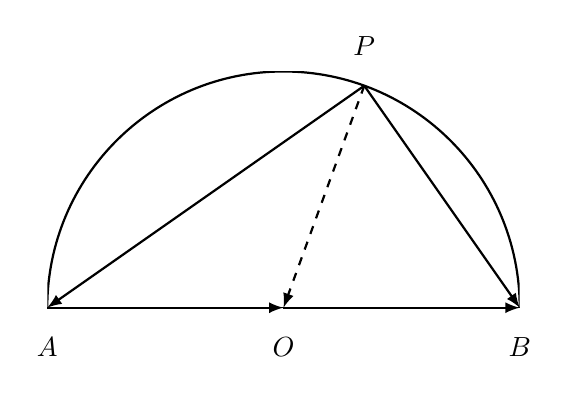
\begin{tikzpicture}[scale=1]
\begin{scope}
    \clip (-3,0) rectangle (3,3);
    \draw[black,thick] (0,0) circle(3);
    \draw[black,thick] (-3,0) -- (3,0);
\end{scope}

\draw[black,thick] [-latex, black, thick] ({3*cos(70)}, {3*sin(70)}) -- (3,0);
\draw[black,thick] [-latex, black, thick] ({3*cos(70)}, {3*sin(70)}) -- (-3,0);
\draw[black,thick,dashed] [-latex, black, thick] ({3*cos(70)}, {3*sin(70)}) -- (0,0);

\draw[black,thick] [-latex, black, thick] (-3,0) -- (0,0);
\draw[black,thick] [-latex, black, thick] (0,0) -- (3,0);

\node at (-3,-0.5) {\(A\)};
\node at (0,-0.5) {\(O\)};
\node at (3,-0.5) {\(B\)};
\node at ({3*cos(70)}, {3*sin(70)+0.5}) {\(P\)};

\end{tikzpicture}





\newpage
\section*{5. kurssi: Analyyttinen geometria}

\item Ratkaise yhtälö ja epäyhtälöt.
\begin{enumerate}[label=\textbf{\alph*)}]
\item \(|2x-1|=21\)
\item \(|x-1|\leq 100\)
\item \(|3x+1|>|x-1|\)
\end{enumerate}

\item Pistejoukko koostuu pisteistä, joiden etäisyys origosta on kaksinkertainen verrattuna niiden etäisyyteen pisteestä \((1,2)\). Määritä pistejoukon yhtälö ja tutki, kuuluuko piste \((4,5)\) pistejoukkoon.

\item Määritä pisteiden \(A=(1,1)\) ja \(B=(2,3)\) välisen janan keskinormaalin yhtälö yleisessä muodossa.

\item Tarkastellaan suoraa \(y=ax-1\) parametrin \(a\in \mathbb{R}\) eri arvoilla.
\begin{enumerate}[label=\textbf{\alph*)}]
\item Määritä \(a\) siten, että suora on yhdensuuntainen suoran \(2x+3y-2=0\) kanssa. Mitkä ovat tällöin suorien suuntakulmat?
\item Kuinka suuri on a-kohdan suorien välinen etäisyys?
\end{enumerate}

\item Origokeskiselle ympyrälle, jonka säde on 5, piirretään tangentit pisteestä \((6,6)\). Kuinka suuri on tangenttien välinen kulma?

\item Ympyrä kulkee pisteen \((1,1)\) kautta. Kuinka suuri on kehäpisteiden \((3,4)\) ja \((4,5)\) välisen kaaren pituus?

\item Olkoot \(A=(2,-1)\) ja \(B=(6,3)\). Määritä yhtälö sille pistejoukolle, jonka pisteistä \((x,y)\) katsottuna jana \(AB\) näkyy suorassa kulmassa. Piirrä pistejoukko. \emph{(Vihje: Voit hyödyntää vektoreita.)}

\item Ympyrän keskipiste on \((r,r)\) ja säde \(r\). Asetetaan uusi ympyrä siten, että se sivuaa koordinaattiakseleita ja alkuperäisen ympyrän origonpuoleista neljänneskaarta (kuva). Määritä tämän ympyrän säde. \emph{(yo s07, mukailtu)}

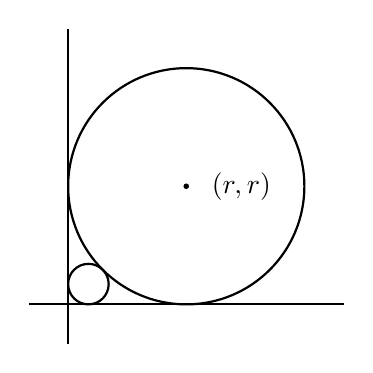
\begin{tikzpicture}
\draw[black,thick] (0,0) circle (1.5cm);
\draw[black,thick] (-1.5,2) -- (-1.5,-2);
\draw[black,thick] (-2,-1.5) -- (2,-1.5);
\draw[black,thick] ({1.5*(sqrt(2)-1)^2-1.5},{1.5*(sqrt(2)-1)^2-1.5}) circle (0.2573cm);

\fill (0,0) circle (1pt);
\node at (0.7, 0) {\((r,r)\)};
\end{tikzpicture}

\newpage
\section*{6. kurssi: Derivaatta}
\item Mitä tarkoitetaan raja-arvolla? Määrää \(\displaystyle \lim_{x\to 2} \dfrac{x^2-4x+4}{x^2-4}\).

\item Ratkaise yhtälö ja epäyhtälö.
\begin{enumerate}[label=\textbf{\alph*)}]
\item \(\dfrac{x}{x-1}-2x=0\)
\item \(\dfrac{4x^3-2x^2-x}{x-2}\leq x\)
\end{enumerate}

\item Miten määritellään funktion jatkuvuus kohdassa \(x=a\)? Millä ehdoilla funktio on jatkuva välillä \([a,b]\)? Anna esimerkki funktiosta, joka on epäjatkuva kohdassa \(x=0\).

\item Miten määritellään reaalifunktion \(f\) derivaatta? Johda määritelmän nojalla funktion \(g(x)=2x^2+x\) derivaattafunktio.

\item Määritä funktioiden derivaatat muuttujan \(x\) suhteen.
\begin{enumerate}[label=\textbf{\alph*)}]
\item \(f(x)=2x^{18}-4x-1\)
\item \(g(x)=ax^2+bx+c\)
\item \(h(x)=\dfrac{2x^2-1}{x+2}-\dfrac{1}{x}\)
\end{enumerate}

\item Tutki funktion \(f(x)=|x^3-2x^2-1|\) kulkua eli määritä, millä väleillä funktio on kasvava ja millä vähenevä sekä määritä ääriarvokohdat.

\item Mittauksessa kappaleen paikalle johdettiin likimääräiskaava \(x(t)=t^4-2t^3+2t\), \(0\leq t \leq 2\). Millä ajanhetkellä kappaleen kiihtyvyys on pienin?

\item Yksikkösäteisen pallon sisälle asetetaan tilavuudeltaan mahdollisimman suuri ympyrälierö. Määritä ympyrälieriön mitat.

\newpage
\section*{7. kurssi: Trigonometriset funktiot}
\item Määritä lausekkeiden arvot yksikköympyrän avulla.

\item Olkoon \(f(t)=\sin(at)\), kun \(t\in \mathbb{R}\). Millä vakion \(a>0\) arvolla lausekkeen \(|f'(t)|\) suurin arvo on 2? \emph{(yo s17)}

\newpage
\section*{8. kurssi: Juuri- ja logaritmifunktiot}
\item Ratkaise yhtälöt.


\newpage
\section*{9. kurssi: Integraalilaskenta}
\item Miten määritellään reaalifunktion \(f\) integraalifunktio?

\newpage
\section*{10. kurssi: Todennäköisyys ja tilastot}
\item Määritä oheisen tilastoaineiston tunnusluvut ...

\newpage
\section*{11. kurssi: Lukuteoria ja todistaminen}
\item Olkoot \(p\) ja \(q\) loogisia lauseita. ...

\item Osoita, että kahden parittoman luvun summa on parillinen, mutta tulo pariton.

\item Todista, että luku \(\sqrt{7}\) on irrationaaliluku.

\item Olkoon luku \(n\) pariton kokonaisluku. Osoita, että tällöin \(n^2 \equiv 1 \pmod{8}\).

\item Etsi sellaiset kokonaislukuparit, joiden summa on 192 ja joiden suurin yhteinen tekijä on 18.
\item Osoita, että mikä tahansa kymmenjärjestelmän luku on jaollinen luvulla 9, jos sen numeroiden summa on jaollinen luvulla 9.
\item Millä numeron \(n\) arvoilla 10-järjestelmän luku \(12n34n567n89n\) on jaollinen luvulla
\begin{enumerate}[label=\textbf{\alph*)}]
\item 3
\item 6
\item 9?
\end{enumerate}
\emph{(yo s2015)}

\item Osoita induktiolla, että \(1^2+2^2+...+n^2=\dfrac{n(n+1)(2n+1)}{6}\), \(n \in \mathbb {N}\).

\item Osoita induktiolla, että \(2^n>n^2\), kun \(n\in \mathbb{N}\) ja \(n\geq 5\).

\item Olkoot \(m\) ja \(n\) positiivisia reaalilukuja, \(n>m\). Osoita, että \(\dfrac{m+1}{n+1}>\dfrac{m}{n}\).
\newpage
\section*{12. kurssi: Numeerisia ja algebrallisia menetelmiä}
\item Määritä yhtälön (jotain) tarkat juuret.

\newpage
\section*{13. kurssi: Differentiaali- ja integraalilaskennan jatkokurssi}
\item Laske integraali $$\int_{-\infty}^{\infty} f(x)\text{ d}x, \ \text{kun }f(x)=\begin{cases} x^4, &\text{jos }x=0\text{ tai }x^4\leq 1/x^4 \\ 1/x^4, &\text{jos }1/x^4\leq x^4. \end{cases}$$

\end{enumerate}

\newpage
\section*{Ratkaisut}

\begin{enumerate}[label=\textbf{\arabic*.}]
\item 
\begin{enumerate}[label=\textbf{\alph*)}]
\item \(\displaystyle 1\frac{2}{3}:2\frac{1}{2}=\frac{5}{3}:\frac{5}{2}=\frac{5}{3}\cdot \frac{2}{5}=\frac{2}{3}\)
\item \(\displaystyle \frac{2^{100}}{4^{50}}=\frac{2^{100}}{(2^2)^{50}}=\frac{2^{100}}{2^{100}}=1\)
\item Luvun \(a\) vastaluku on \(-a\) ja luvun \(\displaystyle b^{-1}=\frac{1}{b}\) käänteisluku on \(b\), joten niiden tulo on \(-ab\).
\item Lukujen tulo on \(\displaystyle \sqrt{2}\cdot \frac{\sqrt{2}}{2}=\frac{\sqrt{2}\cdot \sqrt{2}}{2}=\frac{2}{2}=1\), joten ne ovat toistensa käänteislukuja.
\end{enumerate}

\item Yhtälö saadaan muotoon \((a-3)x=-3a-1\), josta \(\displaystyle x=\frac{-3a-1}{a-3}\). Muuttuja \(x\) ei ole määritelty, kun \(a-3=0\). Yhtälö on siis identtisesti epätosi, kun \(a=3\).

\item 
\begin{enumerate}[label=\textbf{\alph*)}]
\item
$\begin{aligned}[t]
    \displaystyle \frac{3x}{4}+\frac{x}{3}&=1 \qquad \mid \cdot 12 \\
    \frac{12\cdot 3x}{4}+\frac{12\cdot x}{3}&=12 \\
    9x+4x&=12 \\
    13x&=12 \qquad \mid :13 \\
    x&=\frac{12}{13}
\end{aligned}$ 

\item $\begin{aligned}[t]
    \displaystyle 
    2^{4x}&=16 \\
    2^{4x}&=2^4 \\
    4x&=4 \qquad \mid :4 \\
    x&=1
\end{aligned}$ 

\item $\begin{aligned}[t]
    \displaystyle 
    4\cdot 2^x&=\frac{1}{32} \\
    2^2\cdot 2^x&=\frac{1}{2^5} \\
    2^{x+2}&=2^{-5} \\
    x+2&=-5 \\
    x&=-7
\end{aligned}$ 

\item $\begin{aligned}[t]
    \displaystyle 
    2(x-1)-3(x+1)&\leq 1 \\
    2x-2-3x-3&\leq 1 \\
    -x&\leq 6 \qquad \mid \cdot (-1) \\
    x&\geq -6
\end{aligned}$ 
\end{enumerate}
\item Olkoon tuoreen omenan massa \(t\). Kuiva-ainetta on 20 \% eli \(0,20t\). Olkoon kuivatun omenan massa \(k\). Siitä kuiva-ainetta on 90 \% eli \(0,90k\). Kuiva-aineen määrä pysyy vakiona kuivauksessa, joten saadaan yhtälö \(0,20t=0,90k\), mistä \(\displaystyle k=\frac{0,20}{0,90}t\). Koska sokerin määrä pysyy vakiona, on sitä myös kuivatussa omenassa \(0,04t\). Siten sokerin osuus kuivatussa omenassa on \(\displaystyle \frac{0,04t}{\frac{0,20}{0,90}t}=18 \ \%\).

\item Olkoot kuukausimenot \(x\), jolloin vuokran osuus on \(0,05x\).

\begin{enumerate}[label=\textbf{\alph*)}]
\item Uusi vuokra on \(1,02\cdot 0,05x=0,051x\). Siten vuokran osuus kasvoi \(5,1 \ \%-5 \ \%=0,1\) prosenttiyksikköä.
\item Ennen korotusta muihin menoihin kuluu \(0,95x\) ja korotuksen jälkeen \(0,94x\), jotta menot pysyvät samoina. Nyt \(\displaystyle \frac{0,95x}{0,94x}\approx 1,01\), joten muita menoja on pienennettävä 1 \%.
\end{enumerate}

\item 
\begin{enumerate}[label=\textbf{\alph*)}]
\item Jono \((a_n)\) on aritmeettinen, jos ja vain jos erotus \(a_{n+1}-a_n\) on aina jokin luvusta \(n\) riippumaton vakio.

\item Määritelmän nojalla täytyy olla \(3x-(2x-1)=(2x-1)-x\), jolla ei ole ratkaisua. Siten jono ei ole aritmeettinen millään \(x\):n arvolla.
\end{enumerate}

\item Olkoon jonon differenssi \(d\), jolloin \(a_2+3d=a_5\) eli \(4+3d=10\), mistä \(d=2\). Jonon ensimmäinen jäsen on \(a_1=a_2-d=2\) ja sadas jäsen \(a_{100}=2+99\cdot 2=200\). Summaksi saadaan \(\displaystyle S_100=\frac{100\cdot (2+200)}{2}=10 100\).

\item Bakteerien lukumäärät muodostavat geometrisen jonon \((a_n)\), jossa \(a_1=2 000\) ja \(q=1,035\). Olkoon \(n\) aika minuutteina. Yleiselle jäsenelle pätee \(a_n=2 000\cdot 1,035^{n-1}\). Saadaan

\begin{align*}
    \displaystyle 
    2 000\cdot 1,035^{n-1}&=10^6 \qquad \mid :2000 \\
    1,035^{n-1}&=\frac{10^6}{2000} \qquad \mid \lg \\
    (n-1)\cdot \lg 1,035 &= \lg \frac{10^6}{2000} \\
    n&= \frac{\lg \frac{10^6}{2000}}{\lg 1,035}+1 \approx 181,6\text{ (min)}.
\end{align*}
Koska alkuhetki merkittiin ensimmäisen minuutin kohdalle, on kulunut aika 180,6 min. Miljoonan raja on siis ylitetty kello 16.01.

\item Ensimmäiseen jäseneen lisätään 1, toiseen 2 jne. Siten rekursiiviseksi säännöksi voidaan muotoilla \(a_n=a_{n-1}+(n-1)=a_{n-1}+n-1\).

\item Olkoon \(\displaystyle a_n=\frac{1}{2^n}\) ja \(\displaystyle a_{n+1}=\frac{1}{2^{n+1}}\). Jono on geometrinen, koska \(\displaystyle q=\frac{a_{n+1}}{a_n}=\frac{1}{2^{n+1}}:\frac{1}{2^n}=\frac{2^n}{2^{n+1}}=\frac{1}{2}\). Sen ensimmäinen jäsen on \(\displaystyle a_1=\frac{1}{2^1}=\frac{1}{2}\). Summaksi saadaan nyt \(\displaystyle \sum_{n=1}^{100} {\frac{1}{2^n}}=\frac{1/2 \cdot (1-(1/2)^{100})}{1-1/2}=1-\frac{1}{2^{100}}\).


\item 
\begin{enumerate}[label=\textbf{\alph*)}]
\item \(P(x)-Q(x)=x-1-(x^2+1)=x-1-x^2-1=x^2+x-2\)
\item \(P(x)\cdot Q(x)=(x-1)(x^2+1)=x^3+x-x^2-1=x^3-x^2+x-1\)
\item \(P(x)^2=(x-1)^2=x^2-2x+1\)
\end{enumerate}

\item 
\begin{enumerate}[label=\textbf{\alph*)}]
\item \(4x^2-16=(2x-4)(2x+4)\)
\item \(4x^2-4x+1=(2x-1)^2\)
\end{enumerate}

\item Osoittajan nollakohdat saadaan yhtälöstä \(x^2-3x-4=0\), josta \(\displaystyle x=\frac{-(-3) \pm \sqrt{(-3)^2-4\cdot 1\cdot (-4)}}{2\cdot 1}=\frac{3\pm 5}{2}=\begin{cases} 4 \\ -1 \end{cases}\). Osoittajan tulomuodoksi saadaan \((x-4)(x+1)\). Supistettu muoto on siis \(\displaystyle \frac{(x-4)(x+1)}{x-4}=x+1\).

\item
\begin{enumerate}[label=\textbf{\alph*)}]
\item 
\begin{align}
\displaystyle
x^3+0,008&=0 \\
x^3&=-0,008 \\
x^3&= -\frac{8}{1000} \qquad \mid \sqrt[3]{ } \\
x&=-\frac{2}{10}=-\frac{1}{5}

\end{align}

\item Määritetään vastaavan yhtälön juuret. Saadaan \(2x^2-x-3=0\), josta \(\displaystyle x=\frac{-(-1)\pm \sqrt{(-1)^2-4\cdot 2\cdot (-3)}}{2\cdot 2}=\frac{1\pm 5}{4}=\begin{cases} 3/2 \\ -1 \end{cases}\). Funktion kuvaaja on ylöspäin aukeava paraabeli, joten se on positiivinen muualla paitsi nollakohtiensa välillä. Siten yhtälön ratkaisu on \(x\leq -1 \vee x\geq \frac{3}{2}\).

\item Määritetään vastaavan yhtälön juuret. Saadaan \(x^3-x=0\Leftrightarrow x(x^2-1)=0\Leftrightarrow x(x-1)(x+1)=0\), josta \(x=0 \vee x=1 \vee x=-1\). Merkkikaavion nojalla epäyhtälö toteutuu, kun (jotain...)
\end{enumerate}

\item Polynomilla on tekijä \(x-1\), joten sillä on nollakohta \(x=1\). Täytyy siis olla \(2a\cdot 1^2+1-1=0\), josta \(a=0\). Kysytty polynomi on \(f(x)=x-1\), jolla on ensimmäisen asteen funktiona vain yksi nollakohta, \(x=1\).

\item 
\begin{enumerate}[label=\textbf{\alph*)}]
\item Funktio saadaan nyt muotoon \(f(x)=x^3+2x^2+x\), ja sen nollakohdat saadaan yhtälöstä \(x^3+2x^2+x=0\Leftrightarrow x(x^2+2x+1)=0\). Nyt \(x=0\) tai \(\displaystyle x=\frac{-2\pm \sqrt{2^2-4\cdot 1\cdot 1}}{2\cdot 1}=\frac{-2}{2}=-1\).

\item Nyt \(f(x)=tx^3+2x^2+x=x(tx^2+2x+1)\). Funktiolla on aina nollakohta \(x=0\), ja muut nollakohdat saadaan yhtälöstä \(tx^2+2x+1=0\), jolla tulee olla kaksi eri suurta ratkaisua \(\neq 0\). Täytyy olla \(D>0\) eli \((2t)^2-4\cdot t\cdot 1>0\Leftrightarrow 4t^2-4t>0\). Vastaavan yhtälön juuret saadaan yhtälöstä \(4t^2-4t=0\Leftrightarrow 4t(t-1)=0\), josta \(t=0\) tai \(t=1\). Kuvaaja on ylöspäin aukeava paraabeli, joten ehto toteutuu muualla paitsi nollakohtien välissä. (kuvaaja tähän)
\end{enumerate}

\item Funktioiden kuvaajat leikkaavat, kun \(f(x)=g(x)\Leftrightarrow ax^2+4x-1=x^2+x-a\). Yhtälö saadaan muotoon \((a-1)x^2+3x+(a-1)=0\). Koska leikkauspisteitä tulee olla tasan yksi, täytyy olla \(D=0\) eli \(3^2-4\cdot (a-1)\cdot(a-1)=0\), mistä saadaan \(\displaystyle a=\pm \frac{5}{2}\).

\item Piirille saadaan ehto \(a+2h\leq 60\) ja pinta-alalle ehto \(ah=100\), josta \(\displaystyle a=\frac{100}{h}\). Sijoittamalla piirin ehtoon saadaan epäyhtälö \(\frac{100}{h}+2h\leq 60\). Kerrotaan tämä luvulla \(h\) (sivun pituutena positiivinen luku), jolloin saadaan \(2h^2 - 60h + 100 \leq 0\). (jatkuu)

\item
\begin{enumerate}[label=\textbf{\alph*)}]
\item Kerrotaan yhtälö \(x=\frac{2}{3}\) puolittain luvulla 3, jolloin sopivaksi polynomiksi saadaan \(P(x)=3x-2\).

\item Neliöidään yhtälö \(x=\sqrt{3}\) puolittain, jolloin polynomiksi saadaan \(Q(x)=x^2-3\).

\item Muokataan yhtälö muotoon \(x-2=\sqrt{3}\) ja neliöidään puolittain, jolloin saadaan \((x-2)^2=3\) ja lopulta polynomiksi \(R(x)=x^2-4x+1\).

\item Neliöidään yhtälö \(x=\sqrt{2}+\sqrt{3}\) puolittain, jolloin saadaan \(x^2=2\sqrt{2}\sqrt{3} + 5\). Tämä sievenee edelleen muotoon \(x^2-5=2\sqrt{6}\). Neliöidään uudelleen puolittain, jolloin saadaan sopivaksi polynomiksi \(S(x)=x^4-10x^2+1\).
\end{enumerate}

\item 
\begin{enumerate}[label=\textbf{\alph*)}]
\item Kolmio on suorakulmainen, jos ja vain jos sen sivujen pituudet toteuttavat Pythagoraan lauseen. Pisin sivu on \(\sqrt{10}\), joten saadaan \(2^2+(2\sqrt{2})^2=(\sqrt{10})^2\). Yhtälö ei toteudu, joten kolmio ei ole suorakulmainen.

\item Sijoittamalla kolmion pinta-alan trigonometriseen kaavaan \(A=\frac{1}{2}\sin{\alpha}ab\) saadaan \(\frac{1}{2}\cdot \sin{\alpha}\cdot 2\cdot 3=2\), josta \(\sin{\alpha}=\frac{2}{3}\). Siis sivujen välinen kulma on \(\alpha \approx 41,8^{\circ}\) tai suplementtikulma \(180^{\circ}-\alpha \approx 138^{\circ}\).
\end{enumerate}

\item
\begin{enumerate}[label=\textbf{\alph*)}]
\item Nyt \(|\bar{a}|=\sqrt{10^2+3^2}=\sqrt{109}\) ja \(|\bar{b}|=\sqrt{3^2+t^2}=\sqrt{t^2+9}\). Ehdoksi saadaan siis \(\sqrt{t^2+9}=\sqrt{109}\), josta ratkeaa \(t=\pm 10\).
\item Täytyy olla \(\bar{a}\cdot \bar{b}=0\) eli \(10\cdot 3+3\cdot t=0\), josta ratkeaa \(t=-10\).
\item On etsittävä \(s\in \mathbb{R}\) siten, että \(\bar{a}=s\bar{b}\). Siis \(10\bar{i}+3\bar{j}=s(3\bar{i}+t\bar{j})\), josta edelleen \(10\bar{i}+3\bar{j}=3s\bar{i}+st\bar{j}\). Saadaan yhtälöpari \(
\begin{cases}
3s=10 \\
st=3
\end{cases}
\), josta \(s=\frac{10}{3}\), \(t=\frac{9}{10}\). Vektorit ovat siis yhdensuuntaiset, kun \(t=\frac{9}{10}\). Koska \(s>0\), ovat vektorit tällöin samansuuntaiset.
\end{enumerate}

\item
\begin{enumerate}[label=\textbf{\alph*)}]
\item Paikkavektori on vektori, jonka alkupiste on origossa. Esim. \(\overline{OP}=2\bar{i}+\bar{j}\).
\item Olkoot \(\bar{u}\) ja \(\bar{v}\) tason suuntavektoreita (kantavektoreita) ja \(A\) jokin tason tunnettu piste, jolloin tason vektoriyhtälö on muotoa \(\overline{OP}=\overline{OA}+s\bar{u}+t\bar{v}\), \(s,t\in \mathbb{R}\). Sijoittamalla vektoriyhtälöön jotkin \(s\):n ja \(u\):n arvot saadaan jonkin tason pisteen \(P\) paikkavektori \(\overline{OP}\). Esim. \(\overline{OP}=\bar{i}+\bar{j}+\bar{k}+s(2\bar{i}-\bar{j}+\bar{k})+t(3\bar{i}-4\bar{j}+5\bar{k})\).
\item Jaetaan vektori \(\bar{a}\) vektoreiden \(\bar{b}\) ja \(\bar{c}\) suuntaisiin komponentteihin, jolloin on oltava luvut \(r,s\in \mathbb{R}\) siten, että \(\bar{a}=r\bar{b}+s\bar{c}\). Komponenttiesityksen yksikäsitteisyydellä tarkoitetaan sitä, että on olemassa vain yhdet tällaiset luvut \(r\) ja \(s\). Esim. vektori \(\bar{d}\) voidaan esittää muodossa \(\bar{d}=\bar{i}+2\bar{j}\), jossa tehty komponenttijako on yksikäsitteinen.
\item Vektori \(\bar{a}\) ja sen suuntainen yksikkövektori \(\bar{a}^0\) ovat yhdensuuntaisia, ja lisäksi yksikkövektorin \(\bar{a}^0\) pituus on 1. Esim. vektorin \(\bar{b}=\bar{i}+\bar{j}\) pituus on \(|\bar{b}|=\sqrt{1^2+1^2}=\sqrt{2}\), jolloin sen suuntainen yksikkövektori \(\bar{b}^0=\frac{1}{\sqrt{2}}\bar{i}+\frac{1}{\sqrt{2}}\bar{j}\).
\end{enumerate}

\item
\begin{enumerate}[label=\textbf{\alph*)}]
\item Suoran suuntavektoriksi käy esim. \(\overline{BA}=(60-10)\bar{i}+(50-5)\bar{j}+(40-20)\bar{k}=50\bar{i}+45\bar{j}+20\bar{k}\). Lisäksi \(\overline{OA}=60\bar{i}+50\bar{j}+40\bar{k}\). Tällöin suoran vektoriyhtälö on \(\overline{OP}=60\bar{i}+50\bar{j}+40\bar{k}+t(50\bar{i}+45\bar{j}+20\bar{k})\), \(t\in \mathbb{R}\).

\item Muodostetaan aluksi suoran parametriesitys. Sieventämällä vektoriyhtälöstä päästään muotoon \(\overline{OP}=(60+50t)\bar{i}+(50+45t)\bar{j}+(40+2t)\bar{k}\), josta saadaan parametriesitys \(
\begin{cases}
x=60+50t \\
y=50+45t \\
z=40+2t 
\end{cases}
\), \(t\in \mathbb{R}\). Kone koskettaa \(xy\)-tasoa, kun \(z=0\). Tällöin \(40+2t=0\), josta saadaan \(t=-20\). Nyt saadaan \(x=60+50\cdot (-20)=-940\) ja \(y=50+45\cdot (-2)=-850\). Kysytty piste on siis \((-940,-850,0)\).

\item Suuntavektorin projektio \(xy\)-tasolle on \(\bar{a}=60\bar{i}+50\bar{j}\). Lentokoneen ja \(xy\)-tason välinen kulma on vektoreiden \(\bar{a}\) ja \(\overline{BA}\) välinen kulma. Nyt saadaan
\end{enumerate}

\item Nyt \((\bar{a}+\bar{b})\cdot (\bar{a}-\bar{b})=\bar{a}\cdot \bar{a}-\bar{a}\cdot \bar{b}+\bar{a}\cdot \bar{b}-\bar{b}\cdot \bar{b}=\bar{a}\cdot \bar{a}-\bar{b}\cdot \bar{b}\). Koska vektorin pistetulo itsensä kanssa on sen pituuden neliö, on \(\bar{a}\cdot \bar{a}=1^2=1\) ja \(\bar{b}\cdot \bar{b}=(\sqrt{2})^2=2\). Siis \((\bar{a}+\bar{b})\cdot (\bar{a}-\bar{b})=1-2=-1\).

\item Yhdistämällä ympyröiden keskipisteet janoilla muodostuu tasasivuinen kolmio, jonka sivuna on ympyrän halkaisija. Kolikoiden väliin jäävän alueen pinta-ala saadaan kolmion pinta-alan ja kolmen ympyräsektorin pinta-alojen erotuksena. Nyt \(A_\mathrm{kolmio}=\frac{(2,325\text{ cm})^2\cdot \sqrt{3}}{4}\) ja \(A_\mathrm{sektorit}=3\cdot \frac{60^{\circ}}{360^{\circ}}\cdot \pi \cdot (2,325\text{ cm}/2)^2\). Kolikoiden väliin jäävän alueen pinta-ala on \(A=A_\mathrm{kolmio}-A_\mathrm{sektorit}\approx 0,2179\text{ cm}^2\).

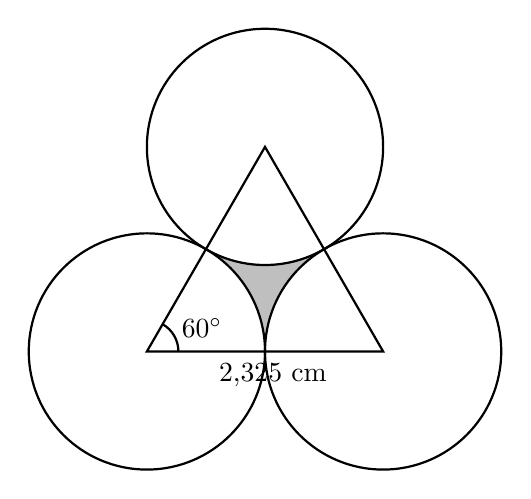
\begin{tikzpicture}
\fill[lightgray] (0.8,0) rectangle (2.2,1.6);
\fill[white] (0,0) circle (1.5cm);
\fill[white] (3,0) circle (1.5cm);
\fill[white] (1.5,{sqrt(9-1.5^2)}) circle (1.5cm);

\draw[black,thick] (0,0) circle (1.5cm);
\draw[black,thick] (3,0) circle (1.5cm);
\draw[black,thick] (1.5,{sqrt(9-1.5^2)}) circle (1.5cm);

\draw[black,thick] (0,0) -- (3,0) -- (1.5,{sqrt(9-1.5^2)}) -- cycle;

\draw[black,thick] (0.4,0) arc (0:60:0.4cm);
\node at (0.7,0.3) {\(60^{\circ}\)};

\node at (1.6,-0.3) {2,325 cm};

\end{tikzpicture}

\item Nyt \(\overline{PB}=\overline{PO}+\overline{OB}\) ja \(\overline{PA}=\overline{PO}-\overline{AO}\). Koska \(\overline{AO}=\overline{OB}\), voidaan merkitä \(\overline{PA}=\overline{PO}-\overline{OB}\). Jännevektoreiden pistetulo on \(\overline{PB}\cdot \overline{PA}=(\overline{PO}+\overline{OB})\cdot (\overline{PO}-\overline{OB})=\overline{PO}\cdot \overline{PO}-\overline{PO}\cdot \overline{OB}+\overline{PO}\cdot \overline{OB}-\overline{OB}\cdot \overline{OB}=\overline{PO}\cdot \overline{PO}-\overline{OB}\cdot \overline{OB}\). Vektorin pistetulo itsensä kanssa on sen pituuden neliö. Koska ympyrän säteinä vektoreilla \(\overline{PO}\) ja \(\overline{OB}\) on sama pituus \(r\), saadaan lopulta \(\overline{PB}\cdot \overline{PA}=r^2-r^2=0\), mistä kohtisuoruus seuraa.

\item Olkoon maailman väestö \(a\) vuonna 1995. Internetin käyttäjiä oli silloin \(0,004a\). Vuonna 2017 maailman väestö oli \(1,3a\) ja Internetin käyttäjiä \(0,496\cdot 1,3a=0,6448a\). Olkoon Internetin käyttäjien vuosittainen kasvukerroin \(k\), jolloin saadaan \(0,004a\cdot k^{22}=0,6448a\). Tästä ratkeaa \(k\approx 1,26\). Siis Internetin käyttäjien määrä on kasvanut vuosittain noin 26 \%.

\item 
\begin{enumerate}[label=\textbf{\alph*)}]
\item Yhtälö \(|2x-1|=21\) saadaan muotoon \(2x-1=\pm 21\), josta \(x=\pm 10\). Siis \(x=10\) tai \(x=-10\).

\item Epäyhtälö \(|x-1|\leq 100\) saadaan muotoon \(-100\leq x-1 \leq 100\), josta \(-99\leq x \leq 101\).

\item Epäyhtälön \(|3x+1|>|x-1|\) molemmat puolet ovat epänegatiivisia, joten se voidaan korottaa puolittain neliöön. Näin saadaan \((3x+1)^2>(x-1)^2\) eli \(8x^2+8x>0 \Leftrightarrow x^2+x>0\). Ratkaisemalla nollakohdat saadaan \(x^2+x=0\Leftrightarrow x(x+1)=0\), josta \(x=0\) tai \(x=-1\). Merkkikaavion tai kuvaajan perusteella havaitaan, että vaadittu ehto toteutuu, kun \(x<-1\) tai \(x>0\).
\end{enumerate}

\item Olkoon mielivaltainen pistejoukon piste \((x,y)\), jolloin saadaan ehto \(\sqrt{x^2+y^2}=2\sqrt{(x-1)^2+(y-2)^2}\). Korottamalla yhtälö puolittain neliöön saadaan \(x^2+y^2=4[(x-1)^2+(y-2)^2]\), josta sieventämällä ja ratkaisukaavalla tai laskimella \(y=\dfrac{1}{3}(8\pm \sqrt{-9x^2+24x+4})\). Sijoitus \((x,y)=(4,5)\) tuottaa epätoden yhtälön, joten piste ei kuulu pistejoukkoon.

\item Pisteiden \(A\) ja \(B\) kautta kulkevan suoran kulmakerroin on \(k_{AB}=\dfrac{3-1}{2-1}=2\). Koska keskinormaali on kohtisuorassa janaa \(AB\) vastaan, määräytyy keskinormaalin kulmakerroin ehdosta \(k_{AB}\cdot k_\text{normaali}=-1\), josta \(k_\text{normaali}=-\dfrac{1}{2}\). Janan \(AB\) keskipiste on \(\left (\dfrac{1+2}{2}, \dfrac{1+3}{2}\right )=(1,5; 2)\). Keskinormaali kulkee tämän pisteen kautta, joten sen yhtälö saadaan muotoon ...

\item yhdensuuntaisuus blah

\item Olkoon koordinaattiakseleiden leikkauspiste \(O=(0,0)\), jolloin \(r\)-säteisen ympyrän keskipisteen etäisyys \(O\):sta on \(\sqrt{r^2+r^2}=\sqrt{2r^2}=\sqrt{2}r\). Olkoon uuden ympyrän säde \(R\). Yhdenmuotoisista kolmioista saadaan, että \(\dfrac{R}{r}=\dfrac{\sqrt{2}r-r-R}{\sqrt{2}r}\). Tästä ratkeaa uuden ympyrän säteeksi \(R=\dfrac{\sqrt{2}-1}{\sqrt{2}+1}r\) eli \(R=(3-2\sqrt{2})r\).

\end{enumerate}
\end{document}
